\chapter{Analysis}
\label{analysis}

The analysis consists of multiple steps, that will be explained in the following.
All parameters for the analysis as well as the features used for the
different random forests can be found in the appendix \ref{sec:app_params}.

\section{Simulated Data and Preprocessing}

Since CTA is not yet fully operational,
the analysis is based entirely on simulated monte carlo (MC) data,
which is seperated into training and test data.
The gamma-/hadron-classifier is trained on diffuse protons and gammas, 
the DISP-/SIGN-models are trained on diffuse gammas.
Evaluation is done on pointlike gamma data as well as a diffuse test set.

Particle shower simulation is done with the software CORSIKA \cite{heck1998corsika}, 
the simulation of the instrument response is done using sim\_telarray \cite{BERNLOHR2008149}.

Simulations parameter nennen? -prod 3 production paper finden!
The simulated initial particle spectrum follows a powerlaw with index $\num{-2}$.

Monte carlo data is simulated and shared across the CTA collaboration, 
our analysis uses the data from the PROD3 simulation of 
the CTA south array. These simulations include more telescopes 
than the array will eventually have in order to compare
different layouts and telescope positions.
The relevant telescopes are chosen in a way, that
the resuting array resembles the earlier mentioned south array (See section \ref{sec:cta}).

The data contains everything the telescopes would measure
at a low level
plus additional MC information, that will not be present at real experiments.
This includes the simulated particle direction, energy and type.
This ground-truth or MC-truth allows to quantify the effectiveness of the 
algorithms by comparing the predictions with the MC-truth values.

At the lowest available level the data consists of uncalibrated waveforms 
in the camera pixels.

The choice of parameters for the low level processing (preprocessing)
is based on values from earlier studies, such as \cite{kai_diss}.

To adress a specific event, the event information will be split into
three layers, that will be saved as separate dataframes, denoted with the keys:
\begin{enumerate}
    \item{$runs$: This contains non-event-specific information about the monte carlo run, e.g.
    spectral\_index, particle injection height, ...}
    \item{$array\_events$: Any shower that triggered the array at some point 
    is considered to be an array event.
    Array-level features consist of array-wide shared event information 
    (e.g. number of triggered telescopes, average intensity),
    reconstructed high-level features of the primary particle (e.g. energy, source position) and the 
    event specific monte carlo information to compare the reconstructed values against.}
    \item{$telescope\_events$: This includes how a specific telescope has seen the shower and
    contains information about the telescope itself (e.g. focal length). Telescope-level features 
    describe the camera image and contain reconstructed features that were retrieved based on 
    the telescope's specific measurements.}
\end{enumerate}

The number of triggered telescopes in an array-event 
will be referred to as the event multiplicity.

\subsection{Features on Telescope Tevel}
\label{sec:tel_analysis}

Processing of the simtel-files is done with the aforementioned ctapipe, starting with 
the calibration of the event. The calibration performs an integration of the waveforms in 
each pixel of a triggered telescopes camera. 

The resulting images get cleaned with a tailcuts approach before they are
used to calculate the image features.
To keep the analysis more comparable to other works and because
of existing parameter choices,
the tailcuts cleaning algorithm is used, which is the default algorithm
for ctapipe at the time of this analysis.

After the image is cleaned, image features get calculated.
This includes the classic hillas parameters among others.
In total the following parameters are being calculated:

\textbf{Hillas Parameters:}

\begin{itemize}
    \item{$x, y$: Coordinates of the image cog}
    \item{$r, \phi$: Coordinates of the cog in polar coordinates}
    \item{$intensity$: Sum of photo-electrons across all pixels}
    \item{$length, width$: Size of the image ellipse}
    \item{$\psi$: Angle between ellipse orientation and main shower axis (?)}
    \item{$skewness, kurtosis$: Higher order image moments along the shower axis}
\end{itemize}

\textbf{Leakage:}

\begin{itemize}
    \item{$leakage\_1\_intensity$: Percentage of photo-electrons in the outer most ring of pixels with respect to the photo-electrons in the whole image}
    \item{$leakage\_1\_pixel$: Percentage of pixels in the outer most ring of pixels with respect to the pixels in the whole image}
    \item{$leakage\_2\_intensity$: Percentage of photo-electrons in the two outer most rings of pixels with respect to the photo-electrons in the whole image}
    \item{$leakage\_2\_pixel$: Percentage of pixels in the two outer most rings of pixels with respect to the pixels in the whole image}
\end{itemize}

\textbf{Concentration:}

\begin{itemize}
    \item{$concentration\_cog$: Percentage of photo-electrons in the three pixels closest to the cog with respect to the photo-electrons in the whole image}
    \item{$concentration\_core$: Percentage of photo-electrons inside the hillas ellipse with respect to the photo-electrons in the whole image}
    \item{$concentration\_pixel$: Percentage of photo-electrons in the brightest pixel with respect to the photo-electrons in the whole image}
\end{itemize}

\textbf{Timing Information:}

\begin{itemize}
    \item{$slope, slope\_err$: Slope and corresponding  error of a linear regression to the pixel-wise pulse times along the main shower axis.}
    \item{$intercept, intercep\_err$: Intercept and corresponding  error of a linear regression to the pixel-wise pulse times along the main shower axis.}
    \item{$deviation$: Root-mean-square deviation between the individual pulse times and the predicted pulse times
        retrieved via the linear regression at the cog. (???)}
\end{itemize}

\textbf{Other:}

\begin{itemize}
    \item{$num\_islands$: Number of individual clusters in the cleaned image.}
    \item{$num\_pixel\_in\_shower$: Number of pixels that survived the cleaning.}
\end{itemize}

\subsection{Features on Array level}  % we dont seperate between 0 and 1 right?
After the image processing of each associated telescope image has been finished,
the predictions of the
HillasReconstructor, which acts as a benchmark for the DISP-calculations, get calculated.

This step leads to the following features on array level:
\begin{itemize}
    \item{$alt, az$: Reconstructed source position}
    \item{$core\_x, core\_y$: Reconstructed core position on the ground}
    \item{$average\_intensity$: Mean intensity over all triggered telescopes}
    \item{$h\_max$: Reconstructed main interaction height}
\end{itemize}

These features are also being added to the telescope level fatures in order to
use them for the machine learning models.

\section{High Level Machine Learning}

High level analysis of the preprocessed data is based on the use of
the aict-tools package \cite{aict-tools} which itself makes use of
scikit-learn \cite{sklearn_api} for the implementation of the machine learning algorithms.
The aict-tools have originally been developed for the FACT-experiment
which is a single IACT. 
For this reason,
adaptions had to be made compared to the status of the project at the start 
of this thesis to perform a stereoscopic analysis. (quelle für fact?)

The algorithm of choice is the random forest algorithm.
Model feature importance is calculated
based on the scikit-learn functionality, which
uses the mean decrease impurity.
For the conclusions drawn in this analysis,
this will be considered to suffice.
For a more general discussion on feature importance estimations see \cite{hastie2017springer}.

Separate models are trained for the tasks of gamma/hadron
separation, DISP estimation and SIGN estimation.

The amount of available data after the earlier 
preprocessing steps is listed in table \ref{tab:events_after_prep}.
(Nur genutzte protonen listen?)

\begin{table}
    \caption{Number of remaining events for each simulated particle type after the
    preprocessing. Pointlike gammas get used for the evaluation, diffuse gammas and protons
    get used for the training of the models, but not all of the available data gets used.}
    \begin{center}
        \begin{tabular}{l r r r}
            %\hline
            & Pointlike Gamma & Diffuse Gamma & Protons \\
            \hline
            MC runs & \num{1113} & \num{17382} &  \num{9273} \\ 
            %\hline
            Array events & \num{955317} & \num{3409290} & \num{4657529} \\
            %\hline
            Telescope events & \num{4554313} & \num{14383270} & \num{20106385} \\
            %\hline
        \end{tabular}
    \end{center}
    \label{tab:events_after_prep}
\end{table}

The data gets split into mutiple dataframes. (WHY?)
The gamma-/hadron-separation model and the DISP-/SIGN-models each get the same
??\% of the available diffuse gamma data for training. ??\% are left out
as a test dataframe.

\subsection{Gamma-/Hadron-Separation}
\label{sec:gh_sep}

For the task of gamma/hadron separation a random forest gets trained
on telescope-event level with the features from \ref{sec:measuring}, including
the features $total\_intensity$, $average\_intensity$, $h\_max$
and $distance\_to\_reconstructed\_core\_position$ from the
HillasReconstructor.
In addition new features get generated, namely:

\begin{enumerate}
    \item $area = width \times length$
    \item $width\_length = 1 - (width/length)$
    \item $log\_size = \log{intensity}$
    \item $log\_size\_area = \log{intensity} / (width \times length)$
\end{enumerate}

A 3-fold cross validation gets used to avoid overfitting.

Performance of the Classifier gets gauged based 
on the AUC.

The single telescope predictions get combined by
taking the mean of the single
predictions to provide a prediction for the complete array-event.

In an analysis of real data, some legitimate events usually get discarded
in the gamma-/hadron-separation step.
Assuming that the misclassified events are in some way not regular or optimal, 
dscarding these events could improve the overall predictions.
For this reason a cut based on the predicted gammaness on the pointlike data
gets applied
and th resulting reconstruction of the source position 
gets compared to the one without the cut applyed.

Selecting a threshold for classification is based on
the $F_{\beta}$-score with $\beta = 0.1$.

% \section{energy estimation}
% Energy estimation can be performed in the same way as the gamma/hadron
% separation. For this task there has been earlier work indicating
% the usefulness of a second machine learning model trained
% on the predictions of the first telesope-level model
% \cite{ba-lars}.

% I am thus going to present results based on either calculating the mean
% of the telescope level predictions and using a second random forest
% to improve the array level prediction.

\subsection{Reconstruction of the Source Position}
\label{sec:source_position}

% The position on the shower axis can be estimated based on 
% the hillas parameters and other image features, as 
% explained in section \ref{sec:measuring}.

The calculation of the DISP is performed with a random
forest regressor model, based on the same features as the gamma-/hadron-separation.,

To resolve the head/tail ambiguity in monoskopic mode,
a second random forest, the SIGN-model, with the same features gets trained
interpreting the two possible sides as two classes.

The monoscopic prediction is then the chosen point in camera coordinates transformed
to sky coordinates (alt/az).
% In our case this is only needed to provide baseline predictions
% on telescope level.

Combining the individual results to an array wide predictions
involves a transformation of the telescope level predictions to
the nominal frame.
The baseline estimation for the stereoscopic reconstruction consists of
calculating the median of the single predictions in this frame and
transforming to the horizon frame afterwards.

Additionaly, an approach inspired by 
what the MAGIC-collaboration does in some of their analyses,
is getting applied.
In the case of the MAGIC-experiment the ambiguity does not
get resolved until the individual results get combined
on the stereo level. The choice of the correct
pair out of the four reconstructed positions can be done either
by calculating the crossing point of both main shower axises
or by calculating the pairwise distances between the positions.
At MAGIC events where the minimum distance between two points is larger than a set threshold
get discarded \cite{ALEKSIC201676}.

The method, where all four distances get calculated, is illustrated in figure \ref{fig:disp_magic}

\begin{figure}
    \centering
    \captionsetup{width=0.9\linewidth}
    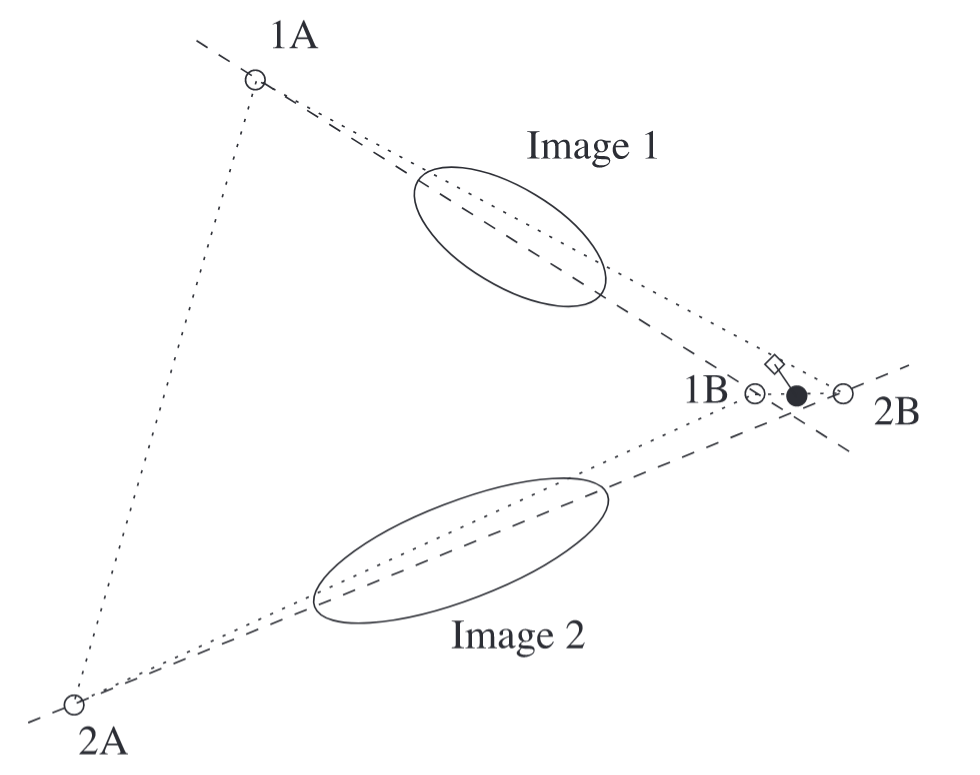
\includegraphics[width=0.9\textwidth]{images/magic_stereo_disp.png}
    \caption{Illustration of the stereoscopic DISP-reconstruction used in MAGIC.
        Two shower ellipses are drawn with the respective main shower axes as dashed lines
        and the two disp predictions each marked as 1A, 1B, 2A, 2B.
        The pairwise distances are displayed by the dotted lines.
        The closest pair is 1B-2B, the resulting prediction is calculated as 
        weighted average between the two points. The true source position is marked with a diamond.
        The illustration has been taken from a study of the Crab Nebula with MAGIC,
        showing the effect of extensive upgrades in 2011-2012 \cite{ALEKSIC201676}.}
    \label{fig:disp_magic}
\end{figure}


Since CTA has more than two telescopes and each array event has a varying number
of associated telescope events, the method needs to be adapted in a scalable way.

The most obvious approach seems to be an iterative one:
For each pair of triggered telescopes, the results get combined
calculating the pairwise distances, as described in figure \ref{fig:disp_magic}. 

Distant events do not get discarded, both because the event count should be kept the same
to compare the results and because choosing an optimal threshold 
is nontrivial especially in the case of different event multiplicities and
telescopes.

From the research done, it seems to have little to no positive effect to weight
the average of the two points based on common image features such as 
the intensity or size, which is why an unweighted mean gets used.

Figure \ref{fig:stereo_disp} illustrates this method for the case of 4 triggered telescopes.

\begin{figure}
    \centering
    \captionsetup{width=0.9\linewidth}
    \begin{subfigure}{0.45\textwidth}
        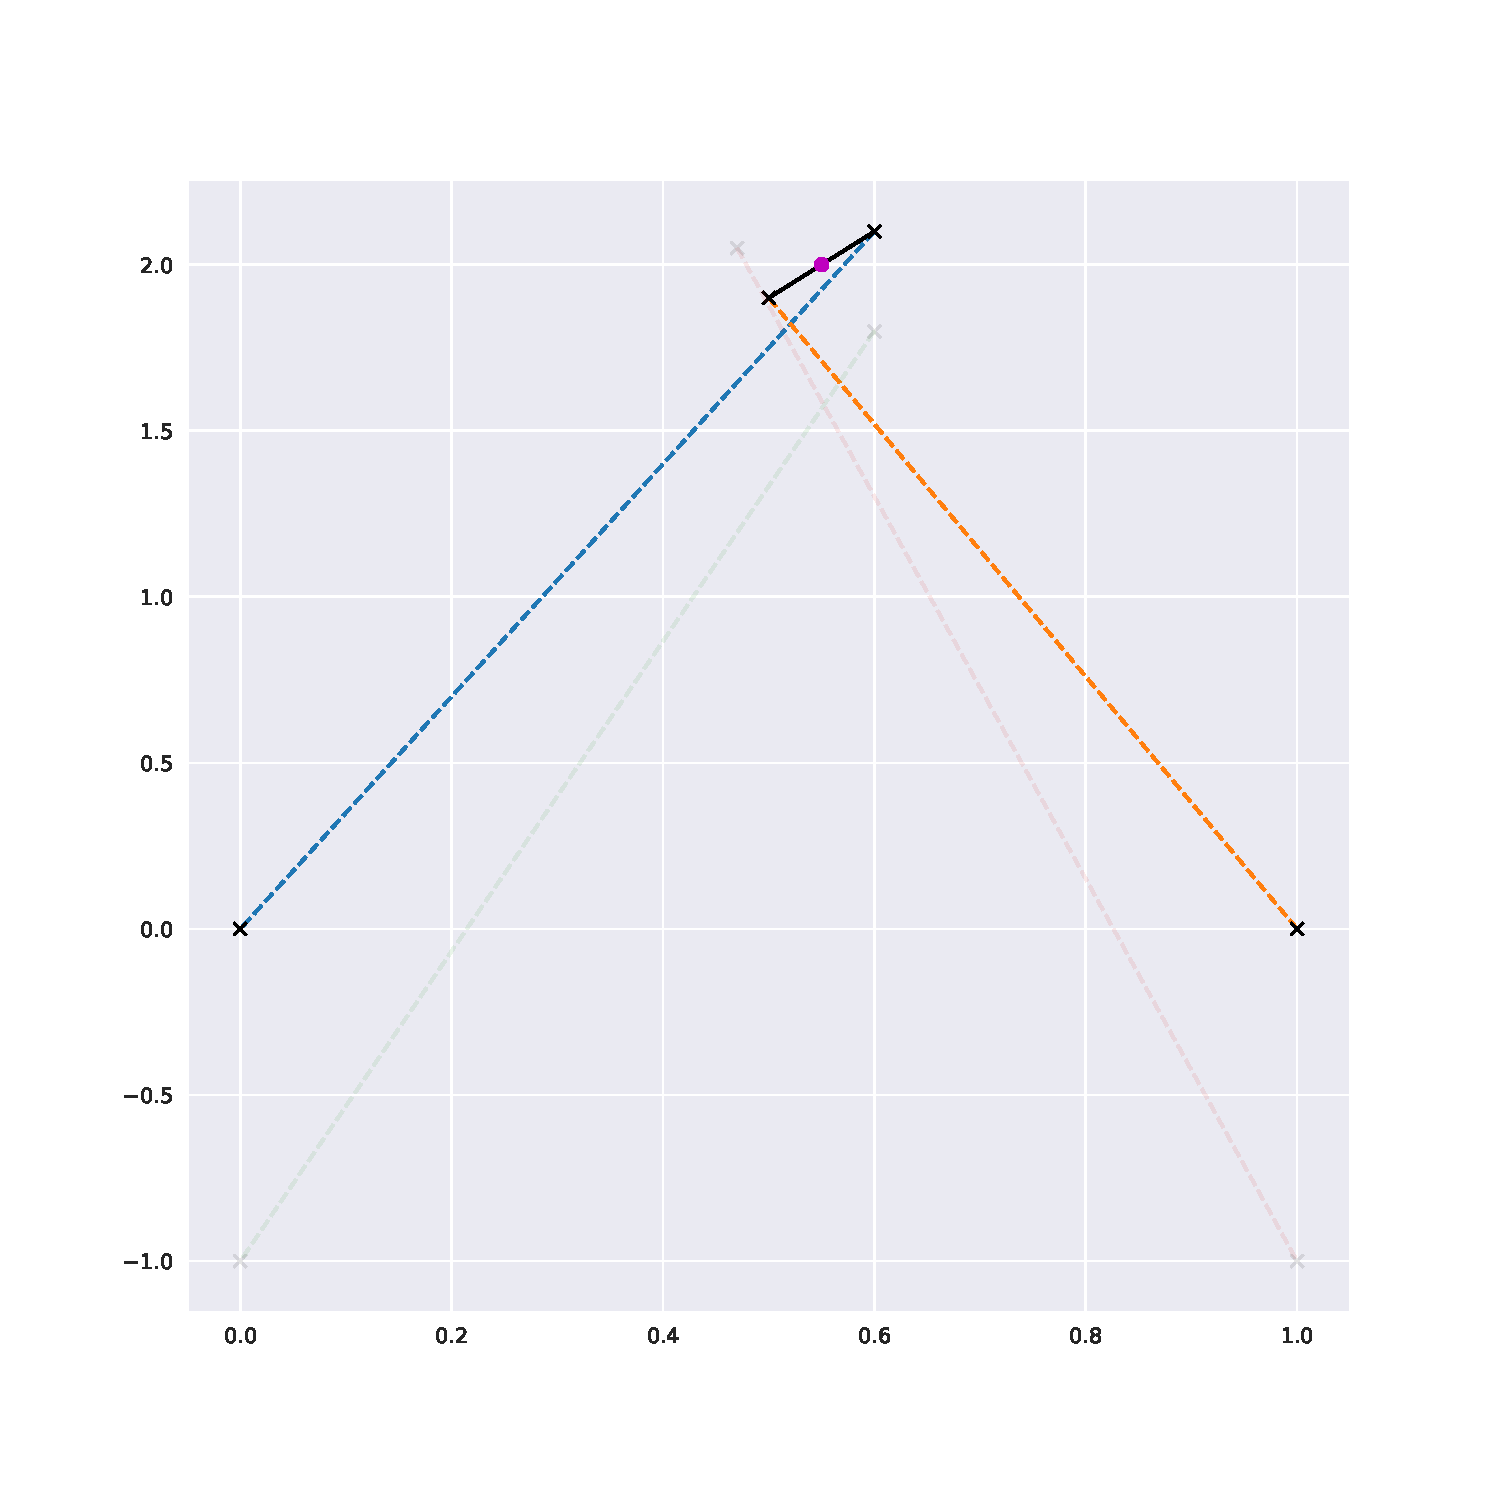
\includegraphics[width=\linewidth]{Plots/stereo_magic_1.pdf}
        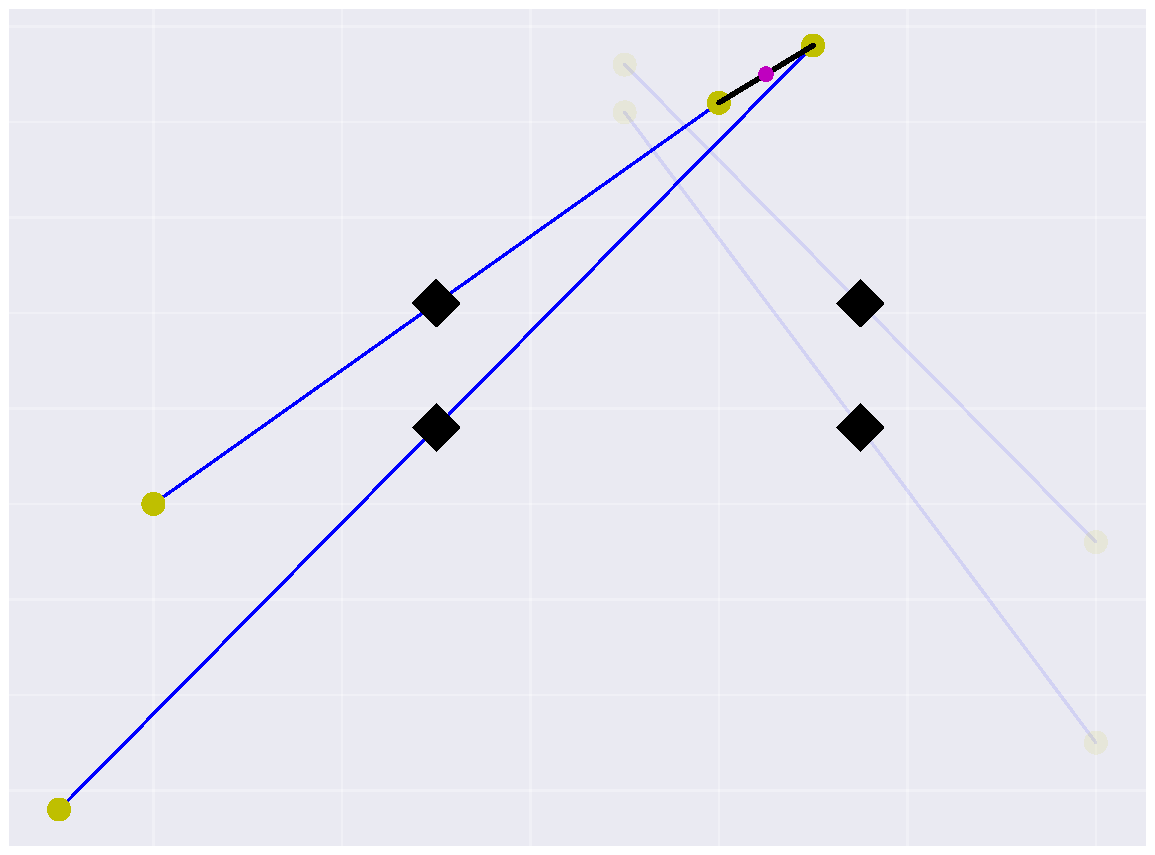
\includegraphics[width=\linewidth]{Plots/stereo_magic_2.pdf}
        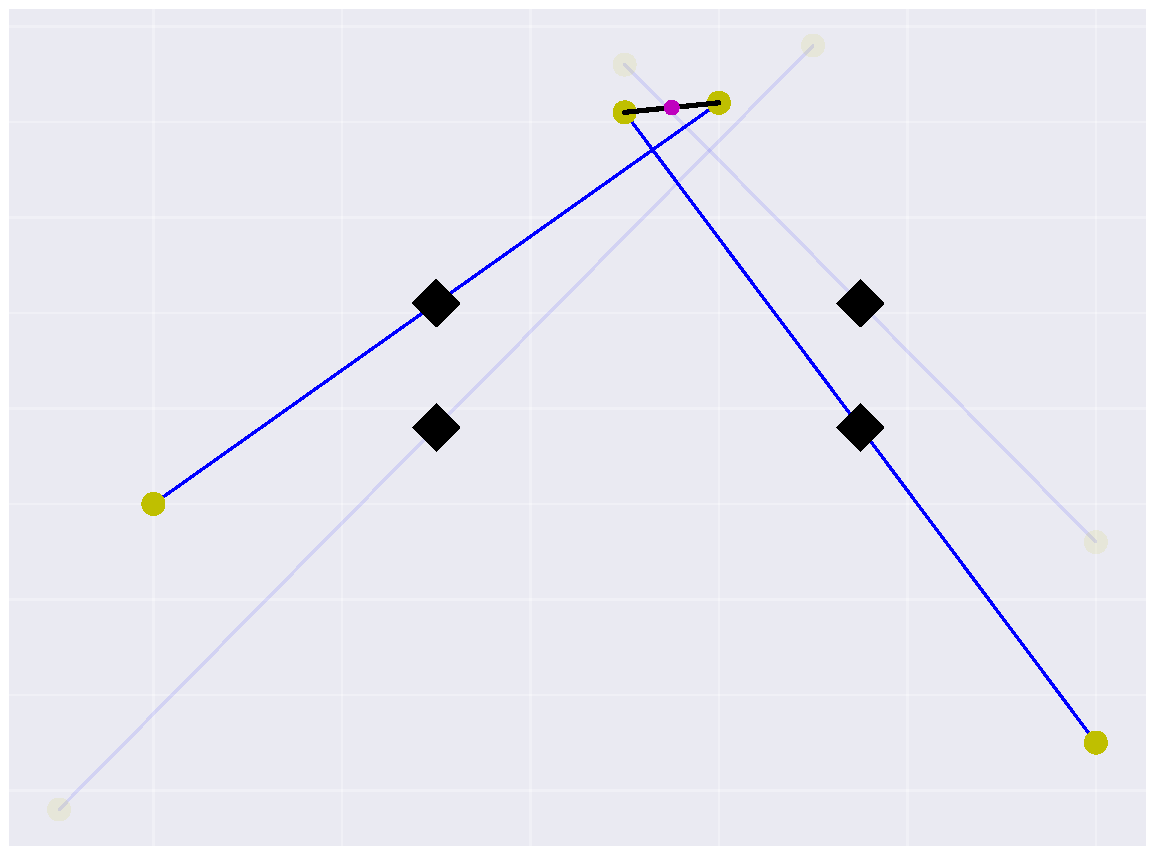
\includegraphics[width=\linewidth]{Plots/stereo_magic_3.pdf}
    \end{subfigure}
    \begin{subfigure}{0.45\textwidth}
        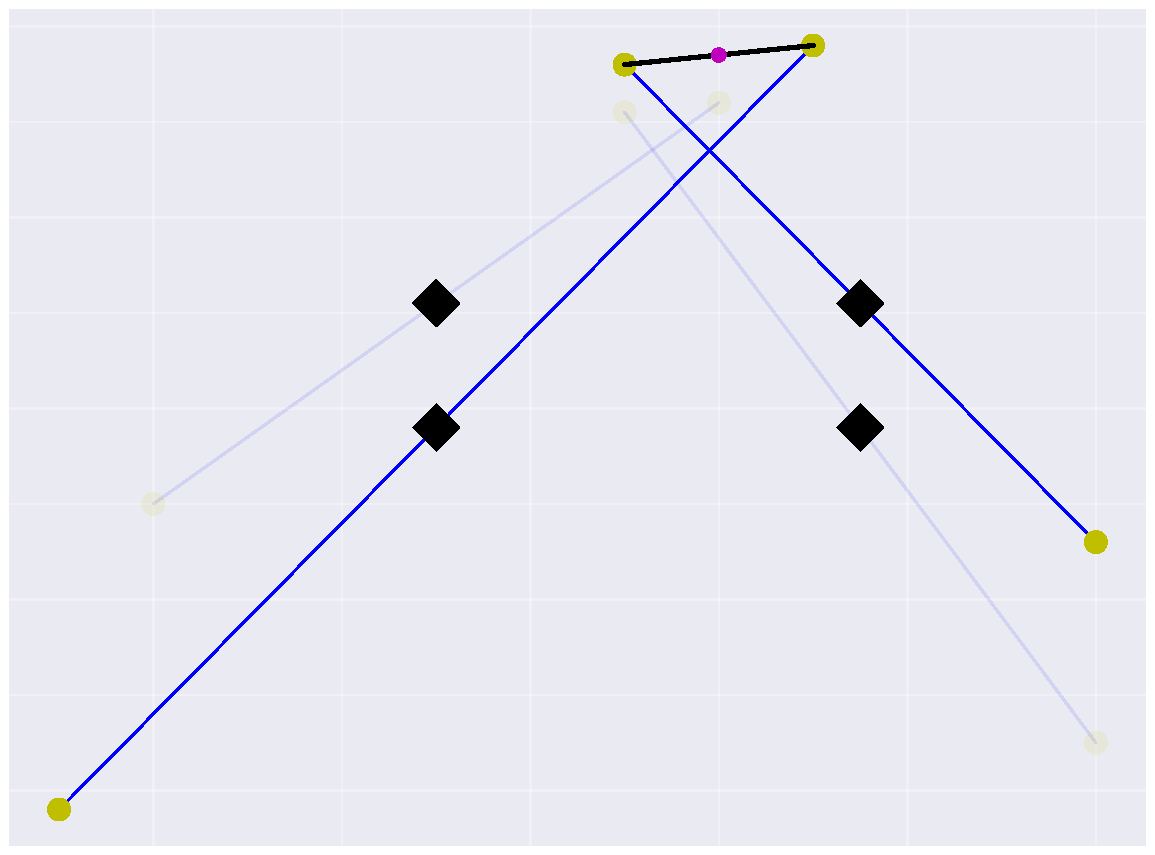
\includegraphics[width=\linewidth]{Plots/stereo_magic_4.pdf}
        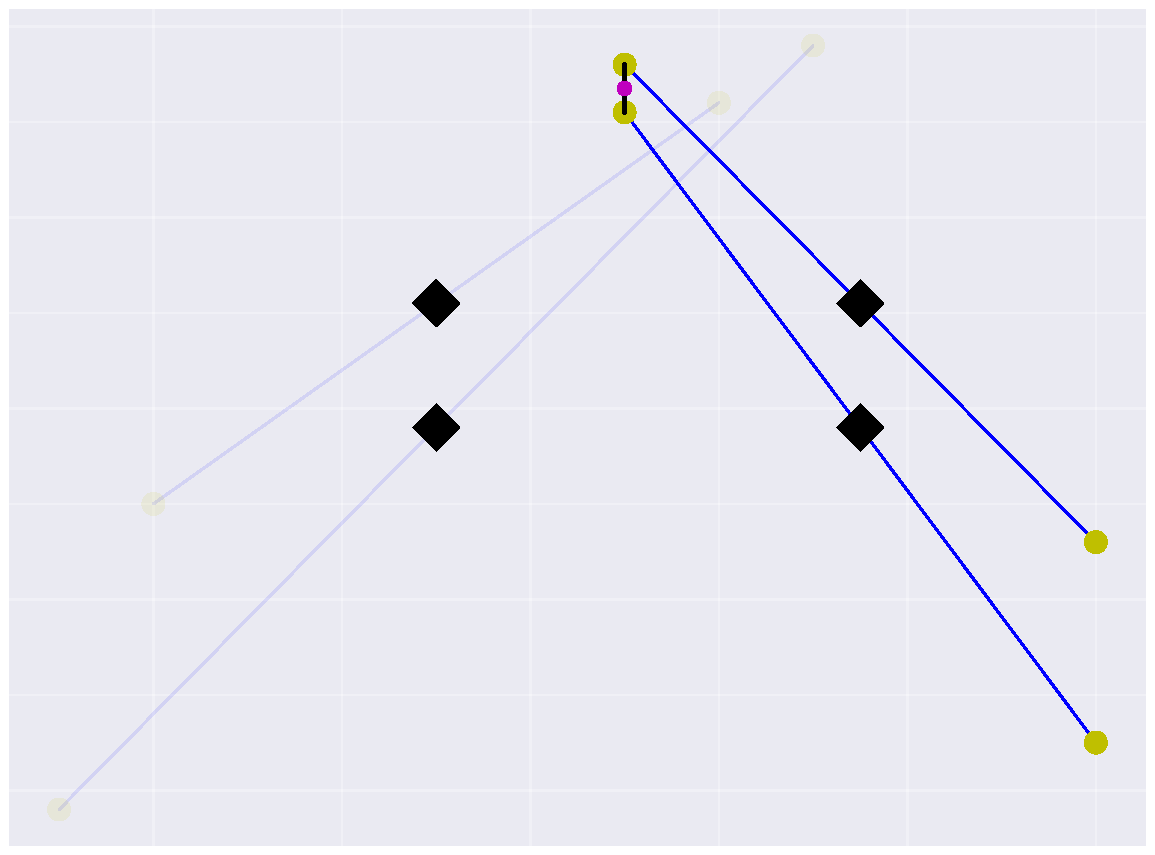
\includegraphics[width=\linewidth]{Plots/stereo_magic_5.pdf} 
        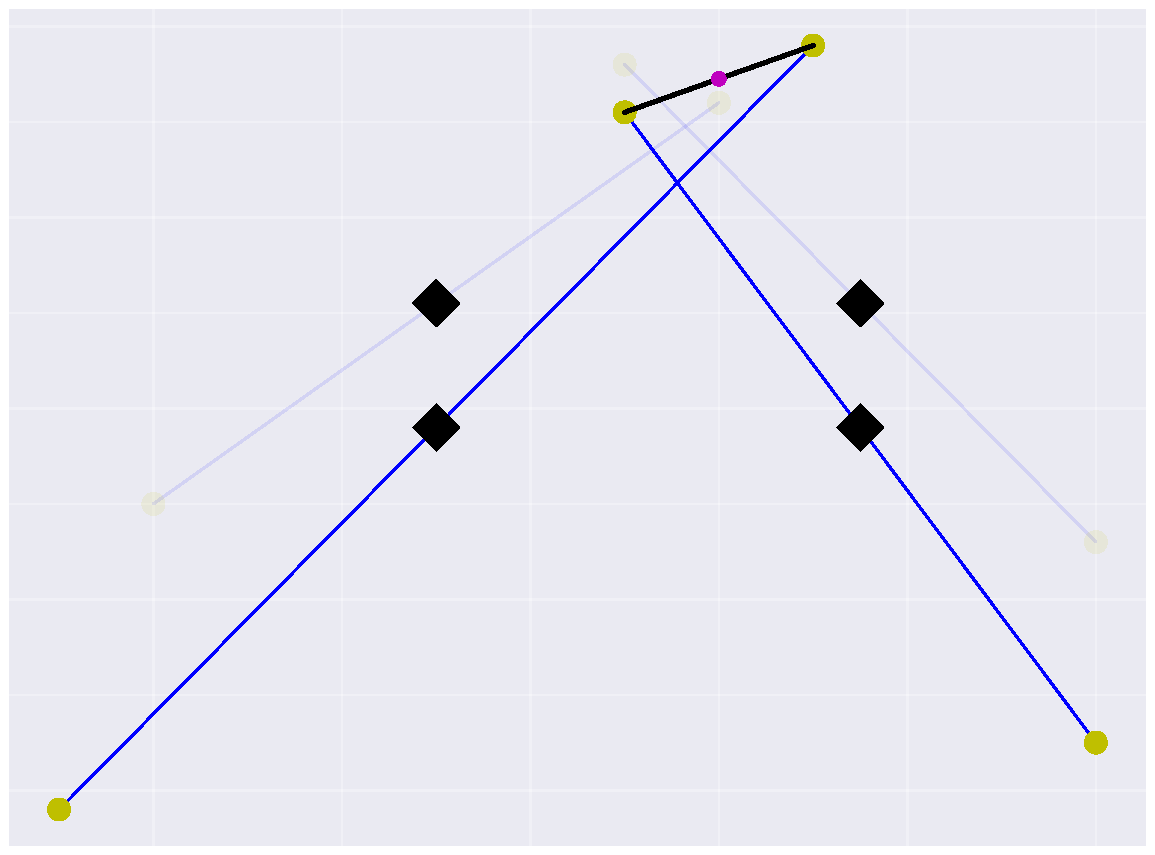
\includegraphics[width=\linewidth]{Plots/stereo_magic_6.pdf} 
    \end{subfigure}
    \caption{
    Illustration of the iterative extension to the stereoscopic magic approach
    with the DISP-predictions as unfilled dots, the intermediate resulting prediction
    as filled dot and the true source position as unfilled diamond.
    Four telescopes have triggered, leading to a total of eight individual DISP-predictions.
    For each pair of telescopes, the four predictions get evaluated according to \cite{ALEKSIC201676}
    without dismissing poor events based on the minimum distance, leading to one 
    intermediate prediction per unique pair.
    Averaging the six intermediate results leads to the final prediction.}
    \label{fig:stereo_disp}
\end{figure}

All intermediate results get saved and averaged to get the final prediction.
In this case taking the median of the pairwise predictions seemed to be more robust
than the mean, weighted or unweighted.

The random forests for the DISP- and SIGN-prediction get trained with a 5-fold cross-validation.

\iffalse
\section{Analysis for a single LST}
Inspired by the current status of CTA with only one LST operating and no MSTs or SSTs
on the north side just yet,
we wanted to add a completely monoskopic analysis.

This is in fact not a real monoscopic analysis and not performed on the north 
side as well. It is merely meant to show that the DISp+SIGn approach works as
expected for the monoscopic LST case.

(MEHR TELESKOPE?? VOLLES MODELL? ALLGEMEIN ALLES NOCH ZIEMLICH WHACKY HIER)
For this reason we chose a single telescope of the simulated data.
Choosing multiple telescopes and treating them as independent events 
would most likely be a valid option as well, although the 
events would not be 100\% uncorellated.

We perform the same analysis for this reduced dataset, leaving out only 
the stereoscopic parts of the analysis.
The machine learning models are expected 
to perform slightly worse as the stereoscopic features are missing.

As explained the HillasReconstructor does not work on a single telescope.
The only source-position predictions we can make and compare are monoscopic 
DISP+SIGN-predictions with the MC truth.
\fi